\documentclass[xcolor=dvipsnames,mathserif,9pt]{beamer} %handout
%\usefonttheme{serif}%{structurebold}%{structuresmallcapsserif}%{serif}

%\input{before_document}
\usepackage{graphicx}
\usepackage{amsmath}
\usepackage{amssymb}
\usepackage[font=footnotesize]{caption} % set the captain font size to 8 (i.e. footnotesize)
\usepackage{subfig} % uses subfloats within a single float MUST after the package {caption}!!
\usepackage{natbib}
%\usepackage{cite} % sort the reference in the article by number or alphabatic
\usepackage{color}
\usepackage{algorithm} % options: boxed [section]
\usepackage{algpseudocode} % for algorithm
%\usepackage{enumerate}
\usepackage{enumitem} % directly use itemize, easily specify indent and everything
\setlist[itemize]{leftmargin=*,label=$\bullet$}%leftmargin=*,itemsep=0pt} %topsep=5pt
\setlist[enumerate]{label={\arabic*)}}
\usepackage{hyperref}
\usepackage{wrapfig}
\usepackage{textpos}
\usepackage{bibentry} % for publication list
\makeatletter\let\saved@bibitem\@bibitem\makeatother % make hyperref and bibentry compatible!!!
\nobibliography*
\usepackage{fancybox}% shadow for image
%\usepackage{empheq} % emphasize equations
\usepackage{bm}
\usepackage{arydshln} % for dashline in table or matrix
\linespread{1.3}
\usepackage{multimedia}

\usepackage{setspace} \setstretch{1.2}

\usepackage{framed}
\colorlet{shadecolor}{black!5}
% for box, page breakable, very good!!
\usepackage[framemethod=TikZ]{mdframed}%
\mdfdefinestyle{myFrame}{%
    linecolor=gray!15!white,%gray
    outerlinewidth=0.1pt,
    roundcorner=3pt,
    skipabove=15pt, % the space before the entire box
    skipbelow=15pt, % the space after the entire box. Please see the figure 2 in the manual, very clear!
    innertopmargin=10pt,%\baselineskip,
    innerbottommargin=10pt,%\baselineskip,
    %innerrightmargin=10pt,
    %innerleftmargin=10pt,
    splittopskip=\baselineskip,
    splitbottomskip=\baselineskip,
    backgroundcolor=gray!10!white,
    frametitlerule=true,
    frametitlebackgroundcolor=gray!20!white,
    frametitleaboveskip=5pt,
    frametitlebelowskip=5pt,
}
\mdfdefinestyle{myAlgo}{%
    linecolor=gray!100!white,%gray
    outerlinewidth=0.1pt,
    roundcorner=3pt,
    skipabove=15pt, % the space before the entire box
    skipbelow=15pt, % the space after the entire box. Please see the figure 2 in the manual, very clear!
    innertopmargin=10pt,%\baselineskip,
    innerbottommargin=10pt,%\baselineskip,
    %innerrightmargin=10pt,
    %innerleftmargin=10pt,
    splittopskip=\baselineskip,
    splitbottomskip=\baselineskip,
    backgroundcolor=gray!0!white,
    frametitlerule=true,
    frametitlebackgroundcolor=gray!20!white,
    frametitleaboveskip=5pt,
    frametitlebelowskip=5pt,
}


\usepackage{tikz}
\usetikzlibrary{calc} % for calculation functions in Tikz let, in commands in Tikz
\usetikzlibrary{shapes} % for block diagram
\usetikzlibrary{chains}
\usetikzlibrary{fit}
\usetikzlibrary{arrows}
\usetikzlibrary{decorations.text} % text along path

\newcommand{\blue}[1]{\textcolor{blue}{#1}}
\definecolor{myred}{RGB}{200,0,0}
\newcommand{\red}[1]{\textcolor{myred}{#1}} %magenta purple
\newcommand{\I}{\mathcal{I}}
\newcommand{\tr}{\mathrm{tr}}
\newcommand{\Null}{\mathrm{Null}}
\newcommand{\Range}{\mathrm{Range}}
\newcommand{\one}{\mathbf{1}}
\newcommand{\rank}{\mathrm{rank}}
\newcommand{\myspan}{\mathrm{span}}
\newcommand{\mydiag}{\mathrm{diag}}
\newcommand{\D}{\mathrm{d}}
\renewcommand{\d}{\mathrm{d}}
\newcommand{\blkdiag}{\mathrm{blkdiag}}
\newcommand{\sgn}{\mathrm{sgn}}
\newcommand{\T}{\mathrm{T}}
\newcommand{\myqed}{\hfill$\blacksquare$}
\newcommand{\ep}{\varepsilon}
\newcommand{\sig}{\mathrm{sig}_a}
%\newcommand{\sigep_}[1]{\sig(\ep_{#1})}
\newcommand{\R}{\mathbb{R}}
\newcommand{\A}{\mathcal{A}}
\newcommand{\G}{\mathcal{G}}
\newcommand{\E}{\mathbb{E}}
\newcommand{\X}{\mathcal{X}}
\newcommand{\V}{\mathcal{V}}
\newcommand{\N}{\mathcal{N}}
\newcommand{\M}{\mathcal{M}}
\renewcommand{\H}{\mathcal{H}}
\renewcommand{\L}{\mathcal{B}}
\renewcommand{\S}{\mathcal{S}}
\newcommand{\xe}{x_{\text{e}}}
%\newcommand{\Null}[1]{\mathrm{Null}\left(#1\right)}
\newcommand{\sk}[1]{\left[#1\right]_\times} % skew symmetric operator
\newcommand{\dia}[1]{\mathrm{diag}\left(#1\right)} % block diagnal matrix
%\renewcommand{\span}[1]{\mathrm{span}\left\{#1\right\}} % ERROR when redefine \span
\newcommand{\Var}{\mathrm{Var}}
\newcommand{\var}{\mathrm{var}}


\graphicspath{{figures/}}

% for tikz, theorem, lemma ... environments have already been declared. You don't need to declare, or you need to use other names than theorem or lemma, such as my_theorem.
%\newtheorem{my_theorem}{Theorem}
%\newtheorem{my_lemma}{Lemma}
\newtheorem{assumption}{Assumption} % necessary for beamer
%\newtheorem{my_remark}{Remark}
\newtheorem{proposition}{Proposition} % necessary for beamer
%\newtheorem{my_corollary}{Corollary}
%\newtheorem{my_example}{Example}
%\newtheorem{my_definition}{Definition}
%\newtheorem{my_problem}{Problem}

%##################################################
\newcommand{\pagetitle}[1]{\textbf{\textcolor{BlueViolet}{$\circ$ #1}}} %!!!
\newcommand{\pagehighlight}[1]{\textbf{\textcolor{Brown}{#1}}} %!!!
\newcommand{\mypause}{\pause} % this is useful for slide show. if you don't want pause any more, just set it as blank
%\newcommand{\mybullet}{\textcolor{BlueViolet}{$\blacksquare$} }%{$\rhd$ }
%\newcommand{\myhighsign}{$\star$ }% the sign to highlight a sentence

%##################################################
% To highlight equation. Example: \begin{align*} \boxed{xxx} \end{align*}
% does not support multiline equations
% put color to \boxed math command
\newcommand*{\boxcolor}{gray}
\makeatletter
\renewcommand{\boxed}[1]{\textcolor{\boxcolor}{%
%\tikz[baseline={([yshift=-1ex]current bounding box.center)}] \node [rectangle, minimum width=1ex,rounded corners,draw] {\normalcolor\m@th$\displaystyle#1$};}}
\tikz[baseline={([yshift=-1ex]current bounding box.center)}] \node [rectangle, minimum width=2ex,rounded corners,draw] {\normalcolor\m@th$\displaystyle#1$};}}
\makeatother

%##################################################
% set my own theme
\def\structureHeight{9mm}
\usetheme[height=\structureHeight]{Rochester}
\usecolortheme[RGB={0,0,128}]{structure}
\setbeamertemplate{items}[circle]%rectangle, triangle,circle
\setbeamertemplate{blocks}[rounded][shadow=true]
\setbeamertemplate{navigation symbols}{}
%\addtobeamertemplate{frametitle}{} % specify the logo
%{
%    \begin{textblock*}{100mm}(.87\textwidth,-\structureHeight)
%        \includegraphics[height=6.6mm,width=3cm,keepaspectratio]{../common_figures_private/westlake_logo.png} % add logo
%    \end{textblock*}
%}
\addtobeamertemplate{frametitle}{\vskip4pt}{} % specify
%\setbeamerfont{frametitle}{size=\large}
\definecolor{mylightgray}{RGB}{240 240 240}
\definecolor{mykhaki}{RGB}{240 230 140}% khaki color
\definecolor{mylightYellow}{RGB}{255,255,224} % light yellow
%\setbeamercolor{beamercolor1}{bg=mylightgray, fg=black}
%\setbeamercolor{beamercolor2}{bg=mylightYellow,fg=black}%{bg=yellow!90!white, fg=black}
% background and foreground color
\setbeamercolor{background canvas}{bg=black!0!white} % background color of every slide! My previous value was black!10!white for my lecture videos!
\setbeamercolor{normal text}{bg=black!10!white} % background color for e.g. theorem environment. When canvas is 10, here it can be 20; the bg for normal text changes the color of hidden text when you use overlay

\setbeamercolor{block title}{bg=mykhaki,fg=black}
\defbeamertemplate{footline}{zsy_frameNumber}
{%
  \hspace{5pt}  \emph{Shiyu Zhao}
  \hspace*{\fill}%
  \usebeamercolor[fg]{page number in head/foot}%
  \insertframenumber\,/\,\inserttotalframenumber \vspace{0pt} \hspace{5pt}
  \vskip5pt
}
\setbeamertemplate{footline}[zsy_frameNumber]
%##################################################
\setbeamercovered{transparent=0} % a good value for transparent text is 20
% when using the overlay commands like \onslide or \uncover, the text will NOT be invisible, instead it will be like transparent
%\pause will also have the transparent effect: command \pause is easy to use: to make it invisible, change the value to zero.



\usepackage{multimedia}
\linespread{1.2}
\newcommand{\hl}{$\triangleright$}
%\newcommand{\blue}[1]{\textcolor{blue}{#1}} % skew symmetric operator

\begin{document}

%%%%%%%%%%%%%%%%%%%%%%%%%%%%%%%%%%%%%%%%%%%%%%%%%%%%%%%%%%%%%%%%%%%%%%%%%%%%%%%%%
% define the author, date etc. information
%\subtitle{Mathematical and Biological Foundation for Reinforcement Learning}
\title{Lecture 2: State Value and Bellman Equation}

\author{Shiyu Zhao
\newline
\newline {\small Department of Artificial Intelligence}
\newline {\small Westlake University}
}
%\logo{\includegraphics[width=1cm,height=1cm,keepaspectratio]{NUSLogo.png}~}
%\date{\today}
\date{}
\subject{}


%%%%%%%%%%%%%%%%%%%%%%%%%%%%%%%%%%%%%%%%%%%%%%%%%%%%%%%%%%%%%%%%%%%%%%%%%%%%%%%%%

{
\setbeamertemplate{footline}{} % remove the frame number of the title page
\begin{frame}
    %\frametitle{Lecture: Networked Dynamic Systems}
    \addtocounter{framenumber}{-1} % discounter the title page, otherwise the frame number starts from 2 instead of 1
    \titlepage % this only gives the author etc. information
\end{frame}
}

%------------------------------------------
\begin{frame}
\frametitle{Outline}
\begin{figure}[h]
  \centering
\includegraphics[width=0.8\linewidth]{fig_bookMap2.pdf}
\end{figure}
\end{frame}
%------------------------------------------
\begin{frame}
\frametitle{Outline}
In this lecture:
\begin{itemize}
\item A core concept: state value
\item A fundamental tool: Bellman equation
\end{itemize}

\end{frame}
%------------------------------------------
\begin{frame}
\frametitle{Outline}
\tableofcontents
\end{frame}
\AtBeginSection[]% put it to the start of each section
{
  \begin{frame}
    \frametitle{Outline}
    \tableofcontents[currentsection]
  \end{frame}
}
%******************************************************************************
\AtBeginSection[]% put it to the start of each section
{
  \begin{frame}
    \frametitle{Outline}
    \tableofcontents[currentsection]
  \end{frame}
}
\section{Motivating examples}
\begin{frame}
\frametitle{Motivating example 1: Why is return important?}

\begin{itemize}
\item What is return? The (discounted) sum of the rewards obtained along a trajectory.

\item Why is return important? See the following examples.
\begin{figure}[h]
  \centering
  \includegraphics[width=0.25\linewidth]{fig_Bellman_demoReturnPolicy1}\qquad
  \includegraphics[width=0.25\linewidth]{fig_Bellman_demoReturnPolicy2}\qquad
  \includegraphics[width=0.28\linewidth]{fig_Bellman_demoReturnPolicy3}
\end{figure}
\end{itemize}

\pause
\begin{itemize}
\item Question: Which policy is the ``best''? Which is the ``worst''?

\begin{itemize}
\pause
\item[-] Intuition: the first is the best and the second is the worst, because of the forbidden area.
\pause
\item[-] Math: can we use mathematics to describe such intuition?

Return could be used to evaluate policies. See the following.
\end{itemize}
\end{itemize}
\end{frame}
%******************************************************************************
\begin{frame}
\frametitle{Motivating example 1: Why return is important?}

\begin{figure}[h]
  \centering
  \includegraphics[width=0.25\linewidth]{fig_Bellman_demoReturnPolicy1}\qquad
  \includegraphics[width=0.25\linewidth]{fig_Bellman_demoReturnPolicy2}\qquad
  \includegraphics[width=0.28\linewidth]{fig_Bellman_demoReturnPolicy3}
\end{figure}

Based on policy 1 (left figure), starting from $s_1$, the discounted return is
\pause
\begin{align*}
\mathrm{return}_1
&=0+\gamma1+\gamma^21+\dots\\
&=\gamma(1+\gamma+\gamma^2+\dots)\\
&=\frac{\gamma}{1-\gamma}
%&=18 \quad(\gamma=0.5)
\end{align*}

\end{frame}
%******************************************************************************
\begin{frame}
\frametitle{Motivating example 1: Why return is important?}

\begin{figure}[h]
  \centering
  \includegraphics[width=0.25\linewidth]{fig_Bellman_demoReturnPolicy1}\qquad
  \includegraphics[width=0.25\linewidth]{fig_Bellman_demoReturnPolicy2}\qquad
  \includegraphics[width=0.28\linewidth]{fig_Bellman_demoReturnPolicy3}
\end{figure}

\textbf{Exercise:} Based on policy 2 (middle figure), starting from $s_1$, what is the discounted return?

\pause
Answer:
\begin{align*}
\mathrm{return}_2
&=-1+\gamma1+\gamma^21+\dots\\
&=-1+\gamma(1+\gamma+\gamma^2+\dots)\\
&=-1+\frac{\gamma}{1-\gamma}
%&=8 \quad(\gamma=0.5)
\end{align*}
\end{frame}
%******************************************************************************
\begin{frame}
\frametitle{Motivating example 1: Why return is important?}

\begin{figure}[h]
  \centering
  \includegraphics[width=0.25\linewidth]{fig_Bellman_demoReturnPolicy1}\qquad
  \includegraphics[width=0.25\linewidth]{fig_Bellman_demoReturnPolicy2}\qquad
  \includegraphics[width=0.28\linewidth]{fig_Bellman_demoReturnPolicy3}
\end{figure}

Policy 3 is stochastic!

\textbf{Exercise:} Based on policy 3 (right figure), starting from $s_1$, the discounted return is

\pause
Answer:
\begin{align*}
\mathrm{return}_3
&=0.5\left(-1+\frac{\gamma}{1-\gamma}\right)+0.5\left(\frac{\gamma}{1-\gamma}\right)\\
&=-0.5+\frac{\gamma}{1-\gamma}
%&=0.5\times 8+0.5\times 18=13 \quad(\gamma=0.5)
\end{align*}

\end{frame}
%******************************************************************************
\begin{frame}
\frametitle{Motivating example 1: Why return is important?}

\begin{figure}[h]
  \centering
  \includegraphics[width=0.25\linewidth]{fig_Bellman_demoReturnPolicy1}\qquad
  \includegraphics[width=0.25\linewidth]{fig_Bellman_demoReturnPolicy2}\qquad
  \includegraphics[width=0.28\linewidth]{fig_Bellman_demoReturnPolicy3}
\end{figure}

In summary, starting from $s_1$,
\begin{align*}
\mathrm{return}_1>\mathrm{return}_3>\mathrm{return}_2
\end{align*}

\begin{itemize}
\pause
\item
The above inequality suggests that the first policy is the best and the second policy is the worst, which is exactly the same as our intuition.
\pause
\item
\blue{Calculating return is important to evaluate a policy.}

\end{itemize}

\end{frame}

%******************************************************************************
\begin{frame}
\frametitle{Motivating example 2: How to calculate return?}

While return is important, how to calculate it?

\begin{figure}[h]
  \centering
  \includegraphics[width=0.25\linewidth]{fig_GridSimple.png}
\end{figure}

\pause
\textbf{Method 1: by definition}

Let $v_i$ denote the return obtained starting from $s_i$ ($i=1,2,3,4$)
\begin{align*}
v_1=r_1+\gamma r_2+\gamma^2 r_3+\dots
\end{align*}
\vspace{-20pt}
\pause
\begin{align*}
v_2=r_2+\gamma r_3+\gamma^2 r_4+\dots\\
v_3=r_3+\gamma r_4+\gamma^2 r_1+\dots\\
v_4=r_4+\gamma r_1+\gamma^2 r_2+\dots
\end{align*}
\end{frame}
%******************************************************************************
\begin{frame}
\frametitle{Motivating example 2: How to calculate return?}

While return is important, how to calculate it? %Consider the following example:

\begin{figure}[h]
  \centering
  \includegraphics[width=0.25\linewidth]{fig_GridSimple.png}
\end{figure}
\textbf{Method 2:}
\begin{align*}
v_1=r_1+\gamma(r_2+\gamma r_3+\dots)=r_1+\gamma v_2
\end{align*}
\vspace{-25pt}
\pause
\begin{align*}
v_2=r_2+\gamma(r_3+\gamma r_4+\dots)=r_2+\gamma v_3\\
v_3=r_3+\gamma(r_4+\gamma r_1+\dots)=r_3+\gamma v_4\\
v_4=r_4+\gamma(r_1+\gamma r_2+\dots)=r_4+\gamma v_1
\end{align*}
\vspace{-20pt}
\pause
\begin{itemize}
\item The returns rely on each other: \blue{Bootstrapping}
\end{itemize}

\end{frame}
%******************************************************************************
\begin{frame}
\frametitle{Motivating example 2: How to calculate return?}
How to solve these equations? Write in the following \blue{matrix-vector form}:
\begin{align*}
\underbrace{\left[
  \begin{array}{c}
    v_1 \\
    v_2 \\
    v_3 \\
    v_4 \\
  \end{array}
\right]}_{\mathbf{v}}
=\left[
  \begin{array}{c}
    r_1 \\
    r_2 \\
    r_3 \\
    r_4 \\
  \end{array}
\right]
+\left[
  \begin{array}{c}
    \gamma v_2 \\
    \gamma v_3 \\
    \gamma v_4 \\
    \gamma v_1 \\
  \end{array}
\right]
\pause
=\underbrace{\left[
  \begin{array}{c}
    r_1 \\
    r_2 \\
    r_3 \\
    r_4 \\
  \end{array}
\right]}_{\mathbf{r}}
+\gamma\underbrace{\left[
   \begin{array}{cccc}
     0 & 1 & 0 & 0 \\
     0 & 0 & 1 & 0 \\
     0 & 0 & 0 & 1 \\
     1 & 0 & 0 & 0 \\
   \end{array}
 \right]}_{\mathbf{P}}
 \underbrace{\left[
\begin{array}{c}
    v_1 \\
    v_2 \\
    v_3 \\
    v_4 \\
  \end{array}
\right]}_{\mathbf{v}}
\end{align*}
\pause
which can be rewritten as
$$\mathbf{v}=\mathbf{r}+\gamma \mathbf{P}\mathbf{v}$$

\pause
This is the Bellman equation (for this specific deterministic problem)!!
\begin{itemize}
\item Though simple, it demonstrates the core idea: the value of one state relies on the values of other states.
\item A matrix-vector form is more clear to see how to solve the state values.
\end{itemize}
\end{frame}
%******************************************************************************
\begin{frame}
\frametitle{Motivating example 2: How to calculate return?}

\textbf{Exercise:} Consider the policy shown in the figure. Please write out the relation among the returns (that is to write out the Bellman equation)

\begin{figure}[h]
  \centering
  \includegraphics[width=0.25\linewidth]{fig_Bellman_demoReturnPolicy1}
\end{figure}
\pause
Answer:
\begin{align*}
v_1&=0+\gamma v_3 \\
v_2&=1+\gamma v_4 \\
v_3&=1+\gamma v_4 \\
v_4&=1+\gamma v_4
\end{align*}
How to solve them? We can first calculate $v_4$, and then $v_3,v_2,v_1$.
\end{frame}
%******************************************************************************
\AtBeginSection[]% put it to the start of each section
{
  \begin{frame}
    \frametitle{Outline}
    \tableofcontents[currentsection]
  \end{frame}
}
\section{State value}
%******************************************************************************
\begin{frame}
\frametitle{Some notations}
Consider the following single-step process:
$$S_t\xrightarrow{A_t} R_{t+1}, S_{t+1}$$
\vspace{-15pt}
\begin{itemize}
\item $t, t+1$: discrete time instances
\item $S_t$: state at time $t$
\item $A_t$: the action taken in state $S_t$
\item $R_{t+1}$: the reward obtained after taking $A_t$
\item $S_{t+1}$: the state transited to after taking $A_t$
\end{itemize}
Note that $S_t,A_t,R_{t+1}$ are all \emph{random variables}.
\end{frame}
%******************************************************************************
\begin{frame}
\frametitle{Some notations}
Consider the following \blue{single-step} process:
$$S_t\xrightarrow{A_t} R_{t+1}, S_{t+1}$$
This step is governed by the following probability distributions:
\begin{itemize}
\item $S_t\rightarrow A_t$ is governed by \textcolor{blue}{$\pi(A_t=a|S_t=s)$}
\item $S_t,A_t\rightarrow R_{t+1}$ is governed by \textcolor{blue}{$p(R_{t+1}=r|S_t=s,A_t=a)$}
\item $S_t,A_t\rightarrow S_{t+1}$ is governed by \textcolor{blue}{$p(S_{t+1}=s'|S_t=s,A_t=a)$}
\end{itemize}
At this moment, we assume we know the model (i.e., the probability distributions)!
\end{frame}
%---------------------------------------------------
\begin{frame}
\frametitle{Some notations}
Consider the following \blue{multi-step} trajectory:
$$S_t\xrightarrow{A_t} R_{t+1}, S_{t+1}\xrightarrow{A_{t+1}} R_{t+2}, S_{t+2}\xrightarrow{A_{t+2}} R_{t+3},\dots$$
\pause
The discounted return is
$$G_t=R_{t+1}+\gamma R_{t+2}+\gamma^2 R_{t+3}+\dots$$
\vspace{-20pt}
\begin{itemize}
\item $\gamma\in(0,1)$ is the discount rate.
\item $G_t$ is also a random variable since $R_{t+1},R_{t+2},\dots$ are random variables.
\end{itemize}

\end{frame}
%******************************************************************************
\begin{frame}
\frametitle{State value}
The expectation (or called expected value or mean) of $G_t$ is defined as the \blue{state-value function} or simply \blue{state value}:
$$v_\pi(s)=\E[G_t|S_t=s]$$

\pause
Remarks:
\begin{itemize}
\item It is a function of $s$. It is a conditional expectation with the condition that the state starts from $s$.
\item It is based on the policy $\pi$. For a different policy, the state value may be different.
\end{itemize}

\vspace{10pt}
\pause
\textbf{Q:} What is the relationship between \blue{return} and \blue{state value}?

\textbf{A:} The state value is the mean of all possible returns that can be obtained starting from a state. If everything - $\pi(a|s)$, $p(r|s,a)$, $p(s'|s,a)$ - is deterministic, then state value is the same as return.
\end{frame}
%******************************************************************************
\begin{frame}
\frametitle{State value}
Example: which policy is good, which is bad?
\begin{figure}[h]
  \centering
  \includegraphics[width=0.25\linewidth]{fig_Bellman_demoReturnPolicy1}\qquad
  \includegraphics[width=0.25\linewidth]{fig_Bellman_demoReturnPolicy2}\qquad
  \includegraphics[width=0.28\linewidth]{fig_Bellman_demoReturnPolicy3}
\end{figure}
Recall the returns obtained from $s_1$ for the three examples:
\begin{align*}
\visible<2->{
v_{\pi_1}(s_1)
&=0+\gamma1+\gamma^21+\dots
=\gamma(1+\gamma+\gamma^2+\dots)
=\frac{\gamma}{1-\gamma}\\}
\visible<3->{
v_{\pi_2}(s_1)
&=-1+\gamma1+\gamma^21+\dots
=-1+\gamma(1+\gamma+\gamma^2+\dots)
=-1+\frac{\gamma}{1-\gamma}\\}
\visible<4->{
v_{\pi_3}(s_1)
&=0.5\left(-1+\frac{\gamma}{1-\gamma}\right)+0.5\left(\frac{\gamma}{1-\gamma}\right)
=-0.5+\frac{\gamma}{1-\gamma}}
\end{align*}

\end{frame}
%******************************************************************************
\AtBeginSection[]% put it to the start of each section
{
  \begin{frame}
    \frametitle{Outline}
    \tableofcontents[currentsection]
  \end{frame}
}
\section{Bellman equation: Derivation}
\begin{frame}
\frametitle{Bellman equation}
\begin{itemize}
\item While state value is important, how to calculate? The answer lies in the Bellman equation.

\pause
\item In a nutshell, the Bellman equation describes the relationship among the values of all states.

\pause
\item Next, we derive the Bellman equation.
\begin{itemize}
\item[-] There is some math, but don't worry as we already have the intuition.
\end{itemize}
\end{itemize}

\end{frame}
%******************************************************************************
\begin{frame}
\frametitle{Deriving the Bellman equation}
Consider a random trajectory:
$$S_t\xrightarrow{A_t} R_{t+1}, S_{t+1}\xrightarrow{A_{t+1}} R_{t+2}, S_{t+2}\xrightarrow{A_{t+2}} R_{t+3},\dots$$
The return $G_t$ can be written as
\begin{align*}
G_{t}
&=R_{t+1}+\gamma R_{t+2}+\gamma^2 R_{t+3}+\dots,\\
&=R_{t+1}+\gamma (R_{t+2}+\gamma R_{t+3}+\dots),\\
&=R_{t+1}+\gamma G_{t+1}
\end{align*}
\pause
Then, it follows from the definition of the state value that
\begin{align*}
v_\pi(s)
&=\E[G_t|S_t=s]\\
&=\E[R_{t+1}+\gamma  G_{t+1} | S_t=s]\\
&=\textcolor{blue}{\E[R_{t+1}|S_t=s]}+\gamma \textcolor{blue}{\E[G_{t+1}|S_t=s]}
\end{align*}
Next, calculate the two terms one by one.
\end{frame}
%******************************************************************************
\begin{frame}
\frametitle{Deriving the Bellman equation}

\textcolor{blue}{First, calculate the first term $\E[R_{t+1}|S_t=s]$:}
\begin{align*}
\E[R_{t+1}|S_t=s]
&=\sum_{a}\pi(a|s)\E[R_{t+1}|S_t=s,A_t=a]\\
&=\sum_{a}\pi(a|s)\sum_{r}p(r|s,a)r
\end{align*}
\pause
Note that
\begin{itemize}
\item This is the mean of \emph{immediate rewards}
%\item $p(r|s,a)$ is given as a priori
\end{itemize}
\end{frame}
%******************************************************************************
\begin{frame}
\frametitle{Deriving the Bellman equation}
\textcolor{blue}{Second, calculate the second term $\E[G_{t+1}|S_t=s]$:}
\begin{align*}
\E[G_{t+1}|S_t=s]
&=\sum_{s'}\E[G_{t+1}|\red{S_t=s},S_{t+1}=s']p(s'|s)\\
&=\sum_{s'}\E[G_{t+1}|S_{t+1}=s']p(s'|s)\\
&=\sum_{s'}v_\pi(s')p(s'|s)\\
&=\sum_{s'}v_\pi(s')\sum_{a}p(s'|s,a)\pi(a|s)
\end{align*}
\pause
Note that
\begin{itemize}
\item This is the mean of \emph{future rewards}
%\item $p(s'|s,a)$ is given as a priori
\item $\E[G_{t+1}|S_t=s,S_{t+1}=s']=\E[G_{t+1}|S_{t+1}=s']$ due to the memoryless Markov property.
\end{itemize}
\end{frame}
%******************************************************************************
\begin{frame}
\frametitle{Deriving the Bellman equation}
Therefore, we have
\begin{align*}%\label{eq_BellmanEquation}
\red{v_\pi(s)}
&=\E[R_{t+1}|S_t=s]+\gamma \E[G_{t+1}|S_t=s],\nonumber\\
&=\textcolor{blue}{\underbrace{\sum_{a}\pi(a|s)\sum_{r}p(r|s,a)r}_{\text{mean of immediate rewards}}+ \underbrace{\gamma\sum_{a}\pi(a|s)\sum_{s'} p(s'|s,a)\red{v_\pi(s')}}_{\text{mean of future rewards}}},\nonumber\\
&=\textcolor{blue}{\sum_{a}\pi(a|s)\left[\sum_{r}p(r|s,a)r+\gamma \sum_{s'} p(s'|s,a)\red{v_\pi(s')}\right]},\quad \forall s\in\S.
\end{align*}

\pause
Highlights:
\begin{itemize}
\item The above equation is called the \emph{Bellman equation}, which characterizes the relationship among the state-value functions of different states.
\item It consists of two terms: the immediate reward term and the future reward term.
\item A set of equations: every state has an equation like this!!!
\end{itemize}
\end{frame}
%******************************************************************************
\begin{frame}
\frametitle{Deriving the Bellman equation}
Therefore, we have
\begin{align*}%\label{eq_BellmanEquation}
\textcolor{red}{v_\pi(s)}
&=\E[R_{t+1}|S_t=s]+\gamma \E[G_{t+1}|S_t=s],\nonumber\\
&=\textcolor{blue}{\underbrace{\sum_{a}\pi(a|s)\sum_{r}p(r|s,a)r}_{\text{mean of immediate rewards}}+ \underbrace{\gamma\sum_{a}\pi(a|s)\sum_{s'} p(s'|s,a)\textcolor{red}{v_\pi(s')}}_{\text{mean of future rewards}}},\nonumber\\
&=\textcolor{blue}{\sum_{a}\pi(a|s)\left[\sum_{r}p(r|s,a)r+\gamma \sum_{s'} p(s'|s,a)\textcolor{red}{v_\pi(s')}\right]},\quad \forall s\in\S.
\end{align*}
Highlights: symbols in this equation
\begin{itemize}
\item $v_\pi(s)$ and $v_\pi(s')$ are state values to be calculated. Bootstrapping!
\item $\pi(a|s)$ is a given policy. Solving the equation is called policy evaluation.
\item $p(r|s,a)$ and $p(s'|s,a)$ represent the dynamic model. What if the model is known or unknown?
\end{itemize}
\end{frame}
%******************************************************************************
\begin{frame}
\frametitle{An illustrative example}

\begin{figure}[h]
  \centering
  \includegraphics[width=0.2\linewidth]{fig_Bellman_demoReturnPolicy1}
\end{figure}

Write out the Bellman equation according to the general expression:
$$v_\pi(s)=\sum_{a}\pi(a|s)\left[\sum_{r}p(r|s,a)r+\gamma \sum_{s'} p(s'|s,a)v_\pi(s')\right]$$

This example is simple because the policy is deterministic.

\pause

First, consider the state value of $s_1$:
\begin{itemize}
\item $\pi(a=a_3|s_1)=1$ and $\pi(a\ne a_3|s_1)=0$.
\item $p(r=0|s_1,a_3)=1$ and $p(r\ne0|s_1,a_3)=0$.
\item $p(s'=s_3|s_1,a_3)=1$ and $p(s'\ne s_3|s_1,a_3)=0$.
\end{itemize}

\pause
Substituting them into the Bellman equation gives
\vspace{-5pt}
$$v_{\pi}(s_1)=0+\gamma v_{\pi}(s_3)$$
\end{frame}
%******************************************************************************
\begin{frame}
\frametitle{An illustrative example}

\begin{figure}[h]
  \centering
  \includegraphics[width=0.2\linewidth]{fig_Bellman_demoReturnPolicy1}
\end{figure}

Write out the Bellman equation according to the general expression:
$$v_\pi(s)=\sum_{a}\pi(a|s)\left[\sum_{r}p(r|s,a)r+\gamma \sum_{s'} p(s'|s,a)v_\pi(s')\right]$$

Similarly, it can be obtained that
\begin{align*}
v_{\pi}(s_1)&=0+\gamma v_{\pi}(s_3), \\
v_{\pi}(s_2)&=1+\gamma v_{\pi}(s_4), \\
v_{\pi}(s_3)&=1+\gamma v_{\pi}(s_4), \\
v_{\pi}(s_4)&=1+\gamma v_{\pi}(s_4).
\end{align*}
\end{frame}
%******************************************************************************
\begin{frame}
\frametitle{An illustrative example}
How to solve them?
\begin{align*}
v_{\pi}(s_1)&=0+\gamma v_{\pi}(s_3), \\
v_{\pi}(s_2)&=1+\gamma v_{\pi}(s_4), \\
v_{\pi}(s_3)&=1+\gamma v_{\pi}(s_4), \\
v_{\pi}(s_4)&=1+\gamma v_{\pi}(s_4).
\end{align*}
\pause
Solve the above equations one by one from the last to the first:
\begin{align*}
v_{\pi}(s_4)&=\frac{1}{1-\gamma},\\
v_{\pi}(s_3)&=\frac{1}{1-\gamma},\\
v_{\pi}(s_2)&=\frac{1}{1-\gamma},\\
v_{\pi}(s_1)&=\frac{\gamma}{1-\gamma}.
\end{align*}
\end{frame}
%******************************************************************************
\begin{frame}
\frametitle{An illustrative example}If $\gamma=0.9$, then
\begin{align*}
v_{\pi}(s_4)&=\frac{1}{1-0.9}=10,\\
v_{\pi}(s_3)&=\frac{1}{1-0.9}=10,\\
v_{\pi}(s_2)&=\frac{1}{1-0.9}=10,\\
v_{\pi}(s_1)&=\frac{0.9}{1-0.9}=9.
\end{align*}
What to do after we have calculated state values? Be patient (calculating action value and improve policy)
\end{frame}
%******************************************************************************
\begin{frame}
\frametitle{Exercise}
\begin{figure}[h]
  \centering
  \includegraphics[width=0.3\linewidth]{fig_Bellman_demoReturnPolicy3}
\end{figure}

\textbf{Exercise:}
$$v_\pi(s)=\sum_{a}\pi(a|s)\left[\sum_{r}p(r|s,a)r+\gamma \sum_{s'} p(s'|s,a)v_\pi(s')\right]$$
\begin{itemize}
\item Write out the Bellman equations for each state.
\item Solve the state values from the Bellman equations.
\item Compare with the policy in the last example.
\end{itemize}

\end{frame}
%******************************************************************************
\begin{frame}
\frametitle{Exercise}
{\small
Answer:
\begin{align*}
v_{\pi}(s_1)&=0.5[0+\gamma v_{\pi}(s_3)]+0.5[-1+\gamma v_{\pi}(s_2)],\\
v_{\pi}(s_2)&=1+\gamma v_{\pi}(s_4), \\
v_{\pi}(s_3)&=1+\gamma v_{\pi}(s_4), \\
v_{\pi}(s_4)&=1+\gamma v_{\pi}(s_4).
\end{align*}
Solve the above equations one by one from the last to the first.
\begin{align*}
v_{\pi}(s_4)&=\frac{1}{1-\gamma}, \quad v_{\pi}(s_3)=\frac{1}{1-\gamma},\quad v_{\pi}(s_2)=\frac{1}{1-\gamma},\\
v_{\pi}(s_1)&=0.5[0+\gamma v_{\pi}(s_3)]+0.5[-1+\gamma v_{\pi}(s_2)],\\
&=-0.5 +\frac{\gamma}{1-\gamma}.
\end{align*}
Substituting $\gamma=0.9$ yields
\begin{align*}
v_{\pi}(s_4)=10,\quad v_{\pi}(s_3)=10,\quad v_{\pi}(s_2)=10,\quad v_{\pi}(s_1)=-0.5+9=8.5.
\end{align*}
Compare with the previous policy. This one is worse.
}
\end{frame}
%******************************************************************************
\AtBeginSection[]% put it to the start of each section
{
  \begin{frame}
    \frametitle{Outline}
    \tableofcontents[currentsection]
  \end{frame}
}
\section{Bellman equation: Matrix-vector form}
\begin{frame}
\frametitle{Matrix-vector form of the Bellman equation}
Why consider the matrix-vector form? Because we need to solve the state values from it!
\begin{itemize}
\pause
\item One unknown relies on another unknown. How to solve the unknowns?
$$\textcolor{red}{v_\pi(s)}=\sum_{a}\pi(a|s)\left[\sum_{r}p(r|s,a)r+\gamma \sum_{s'} p(s'|s,a)\textcolor{red}{v_\pi(s')}\right]$$

\pause
\item Elementwise form: The above \emph{elementwise form} is valid for every state $s\in\S$.
That means there are $|\S|$ equations like this!

\pause
\item Matrix-vector form: If we put all the equations together, we have a set of linear equations, which can be concisely written in a \emph{matrix-vector form}. The matrix-vector form is very elegant and important.
\end{itemize}
\end{frame}
%******************************************************************************
\begin{frame}
\frametitle{Matrix-vector form of the Bellman equation}
Recall that:
$$v_\pi(s)=\sum_{a}\pi(a|s)\left[\sum_{r}p(r|s,a)r+\gamma \sum_{s'} p(s'|s,a)v_\pi(s')\right]$$
Rewrite the Bellman equation as
\begin{align*}%\label{eq_MDP_bellmanequation2}
v_\pi(s)=r_\pi(s)+\gamma \sum_{s'}p_\pi(s'|s)v_\pi(s')
\end{align*}
where
\begin{align*}%\label{eq_MDP_bellmanequation_element}
r_\pi(s)\doteq\sum_{a}\pi(a|s)\sum_{r}p(r|s,a)r,\qquad p_\pi(s'|s)\doteq\sum_{a}\pi(a|s)p(s'|s,a)
\end{align*}

\end{frame}
%******************************************************************************
\begin{frame}
\frametitle{Matrix-vector form of the Bellman equation}

Suppose the states could be indexed as $s_i$ ($i=1,\dots,n$).

For state $s_i$, the Bellman equation is
\begin{align*}
v_\pi(s_i)=r_\pi(s_i)+\gamma  \sum_{s_j}p_\pi(s_j|s_i)v_\pi(s_j)
\end{align*}

\pause
Put all these equations for all the states together and rewrite to a matrix-vector form
\begin{align*}
\textcolor{blue}{v_\pi=r_\pi+\gamma  P_\pi v_\pi}
\end{align*}
where
\begin{itemize}
\item $v_\pi=[v_\pi(s_1),\dots,v_\pi(s_n)]^T\in\R^{n}$
\item $r_\pi=[r_\pi(s_1),\dots,r_\pi(s_n)]^T\in\R^{n}$
\item $P_\pi\in\R^{n\times n}$, where $[P_\pi]_{ij}=p_\pi(s_j|s_i)$, is the \emph{state transition matrix}.
\end{itemize}

\end{frame}
%******************************************************************************
\begin{frame}
\frametitle{Illustrative examples}

If there are four states, $v_\pi=r_\pi+\gamma  P_\pi v_\pi$ can be written out as
\begin{align*}
\resizebox{\columnwidth}{!}{$ % you need to add $ when you use resizebox for equations!
\underbrace{\left[
  \begin{array}{c}
    v_{\pi}(s_1) \\
    v_{\pi}(s_2) \\
    v_{\pi}(s_3) \\
    v_{\pi}(s_4) \\
  \end{array}
\right]}_{v_\pi}
=
\underbrace{\left[
  \begin{array}{c}
    r_\pi(s_1) \\
    r_\pi(s_2) \\
    r_\pi(s_3) \\
    r_\pi(s_4) \\
  \end{array}
\right]}_{r_\pi}
+\gamma
\underbrace{\left[
  \begin{array}{cccc}
    p_\pi(s_1|s_1) & p_\pi(s_2|s_1) & p_\pi(s_3|s_1) & p_\pi(s_4|s_1) \\
    p_\pi(s_1|s_2) & p_\pi(s_2|s_2) & p_\pi(s_3|s_2) & p_\pi(s_4|s_2) \\
    p_\pi(s_1|s_3) & p_\pi(s_2|s_3) & p_\pi(s_3|s_3) & p_\pi(s_4|s_3) \\
    p_\pi(s_1|s_4) & p_\pi(s_2|s_4) & p_\pi(s_3|s_4) & p_\pi(s_4|s_4) \\
  \end{array}
\right]}_{P_\pi}
\underbrace{\left[
  \begin{array}{c}
    v_{\pi}(s_1) \\
    v_{\pi}(s_2) \\
    v_{\pi}(s_3) \\
    v_{\pi}(s_4) \\
  \end{array}
\right]}_{v_\pi}
$}
\end{align*}

\visible<2->{
For the following example:
\begin{figure}[h]
  \centering
  \includegraphics[width=0.25\linewidth]{fig_Bellman_demoReturnPolicy1}
\end{figure}
{\small
\begin{align*}
\left[
  \begin{array}{c}
    v_{\pi}(s_1) \\
    v_{\pi}(s_2) \\
    v_{\pi}(s_3) \\
    v_{\pi}(s_4) \\
  \end{array}
\right]
=
\left[
  \begin{array}{c}
    0 \\
    1 \\
    1 \\
    1 \\
  \end{array}
\right]
+\gamma
\left[
  \begin{array}{cccc}
    0 & 0 & 1 & 0 \\
    0 & 0 & 0 & 1 \\
    0 & 0 & 0 & 1 \\
    0 & 0 & 0 & 1 \\
  \end{array}
\right]
\left[
  \begin{array}{c}
    v_{\pi}(s_1) \\
    v_{\pi}(s_2) \\
    v_{\pi}(s_3) \\
    v_{\pi}(s_4) \\
  \end{array}
\right]
\end{align*}
}
}
\end{frame}
%******************************************************************************
\begin{frame}
\frametitle{Illustrative examples}

If there are four states, $v_\pi=r_\pi+\gamma  P_\pi v_\pi$ can be written out as
\begin{align*}
\resizebox{\columnwidth}{!}{$ % you need to add $ when you use resizebox for equations!
\underbrace{\left[
  \begin{array}{c}
    v_{\pi}(s_1) \\
    v_{\pi}(s_2) \\
    v_{\pi}(s_3) \\
    v_{\pi}(s_4) \\
  \end{array}
\right]}_{v_\pi}
=
\underbrace{\left[
  \begin{array}{c}
    r_\pi(s_1) \\
    r_\pi(s_2) \\
    r_\pi(s_3) \\
    r_\pi(s_4) \\
  \end{array}
\right]}_{r_\pi}
+\gamma
\underbrace{\left[
  \begin{array}{cccc}
    p_\pi(s_1|s_1) & p_\pi(s_2|s_1) & p_\pi(s_3|s_1) & p_\pi(s_4|s_1) \\
    p_\pi(s_1|s_2) & p_\pi(s_2|s_2) & p_\pi(s_3|s_2) & p_\pi(s_4|s_2) \\
    p_\pi(s_1|s_3) & p_\pi(s_2|s_3) & p_\pi(s_3|s_3) & p_\pi(s_4|s_3) \\
    p_\pi(s_1|s_4) & p_\pi(s_2|s_4) & p_\pi(s_3|s_4) & p_\pi(s_4|s_4) \\
  \end{array}
\right]}_{P_\pi}
\underbrace{\left[
  \begin{array}{c}
    v_{\pi}(s_1) \\
    v_{\pi}(s_2) \\
    v_{\pi}(s_3) \\
    v_{\pi}(s_4) \\
  \end{array}
\right]}_{v_\pi}.
$}
\end{align*}
For the following example:
\begin{figure}[h]
  \centering
  \includegraphics[width=0.25\linewidth]{fig_Bellman_demoReturnPolicy3}
\end{figure}
{\footnotesize
\begin{align*}
\left[
  \begin{array}{c}
    v_{\pi}(s_1) \\
    v_{\pi}(s_2) \\
    v_{\pi}(s_3) \\
    v_{\pi}(s_4) \\
  \end{array}
\right]
=
\left[
  \begin{array}{c}
    0.5(0)+0.5(-1) \\
    1 \\
    1 \\
    1 \\
  \end{array}
\right]
+\gamma
\left[
  \begin{array}{cccc}
    0 & 0.5 & 0.5 & 0 \\
    0 & 0 & 0 & 1 \\
    0 & 0 & 0 & 1 \\
    0 & 0 & 0 & 1 \\
  \end{array}
\right]
\left[
  \begin{array}{c}
    v_{\pi}(s_1) \\
    v_{\pi}(s_2) \\
    v_{\pi}(s_3) \\
    v_{\pi}(s_4) \\
  \end{array}
\right].
\end{align*}
}
\end{frame}
%******************************************************************************
\AtBeginSection[]% put it to the start of each section
{
  \begin{frame}
    \frametitle{Outline}
    \tableofcontents[currentsection]
  \end{frame}
}
\section{Bellman equation: Solve the state values}
\begin{frame}
\frametitle{Solve state values}

Why to solve state values?
\begin{itemize}
\item Given a policy, finding out the corresponding state values is called \textcolor{blue}{policy evaluation}!
\item It is a fundamental problem in RL. It is the foundation to find better policies.
\item Therefore, it is important to understand how to solve the Bellman equation.
\end{itemize}

\end{frame}
%******************************************************************************
\begin{frame}
\frametitle{Solve state values}
The Bellman equation in matrix-vector form is
$$v_\pi=r_\pi+\gamma P_\pi v_\pi$$
\begin{itemize}
\pause
\item
The \blue{closed-form solution} is
$$v_\pi=(I-\gamma  P_\pi)^{-1}r_\pi$$
\begin{itemize}
\item[-] The matrix $I-\gamma  P_\pi$ is invertible. See details in my book.
\item[-] We still need to use numerical algorithms to calculate the matrix inverse.
\item[-] Can we avoid the matrix inverse operation? Yes, as shown below.
\end{itemize}
\vspace{10pt}

\pause
\item
An \blue{iterative solution} is
$$v_{k+1}=r_\pi+\gamma  P_\pi v_k$$
This algorithm leads to a sequence $\{v_0,v_1,v_2,\dots\}$.
We can show that
$$v_k\rightarrow v_\pi=(I-\gamma  P_\pi)^{-1}r_\pi, \quad k\rightarrow\infty$$
\end{itemize}
\end{frame}
%******************************************************************************
\begin{frame}
\frametitle{Solve state values (optional)}
{\small
\begin{proof}
Define the error as
$$\delta_k=v_k-v_\pi.$$
We only need to show $\delta_k\rightarrow 0$.
Substituting $v_{k+1}=\delta_{k+1}+v_\pi$ and $v_{k}=\delta_{k}+v_\pi$ into $v_{k+1}=r_\pi+\gamma  P_\pi v_k$ gives
$$\delta_{k+1}+v_\pi=r_\pi+\gamma P_\pi (\delta_k+v_\pi),$$
which can be rewritten as
\begin{align*}
\delta_{k+1}
&=-v_\pi+r_\pi+\gamma P_\pi \delta_k+ \gamma P_\pi v_\pi=\gamma P_\pi \delta_k.
\end{align*}
As a result,
$$\delta_{k+1}=\gamma P_\pi \delta_k=\gamma^2 P_\pi^2 \delta_{k-1}=\dots=\gamma^{k+1} P_\pi^{k+1} \delta_0.$$
Note that $0\le P_{\pi}^k\le1$, which means every entry of $P_{\pi}^k$ is no greater than 1 for any $k=0,1,2,\dots$. That is because $P_{\pi}^k\one=\one$, where $\one=[1,\dots,1]^T$. On the other hand, since $\gamma<1$, we know $\gamma^k\rightarrow0$ and hence $\delta_{k+1}=\gamma^{k+1} P_\pi^{k+1} \delta_0\rightarrow0$ as $k\rightarrow\infty$.
\end{proof}
}
\end{frame}

%******************************************************************************
\begin{frame}
\frametitle{Solve state values}
Examples: $r_{\rm boundary}=r_{\rm forbidden}=-1$, $r_{\rm target}=+1$, $\gamma=0.9$

\begin{itemize}
\item The following are two ``\blue{good}'' policies and the state values. The two policies are different for the top two states in the forth column.
\end{itemize}

\begin{figure}[h!]
  \centering
  \includegraphics[width=0.25\linewidth]{fig_gridPolicy_good.pdf}
  \includegraphics[width=0.25\linewidth]{fig_gridStateValue_good.pdf}\\
  \vspace{10pt}
  \includegraphics[width=0.25\linewidth]{fig_gridPolicy_good1.pdf}
  \includegraphics[width=0.25\linewidth]{fig_gridStateValue_good1.pdf}
\end{figure}

\end{frame}
%******************************************************************************
\begin{frame}
\frametitle{Solve state values}
Examples: $r_{\rm boundary}=r_{\rm forbidden}=-1$, $r_{\rm target}=+1$, $\gamma=0.9$
\begin{itemize}
\item The following are two ``\blue{bad}'' policies and the state values. The state values are less than those of the good policies.
\end{itemize}

\begin{figure}[h!]
  \centering
  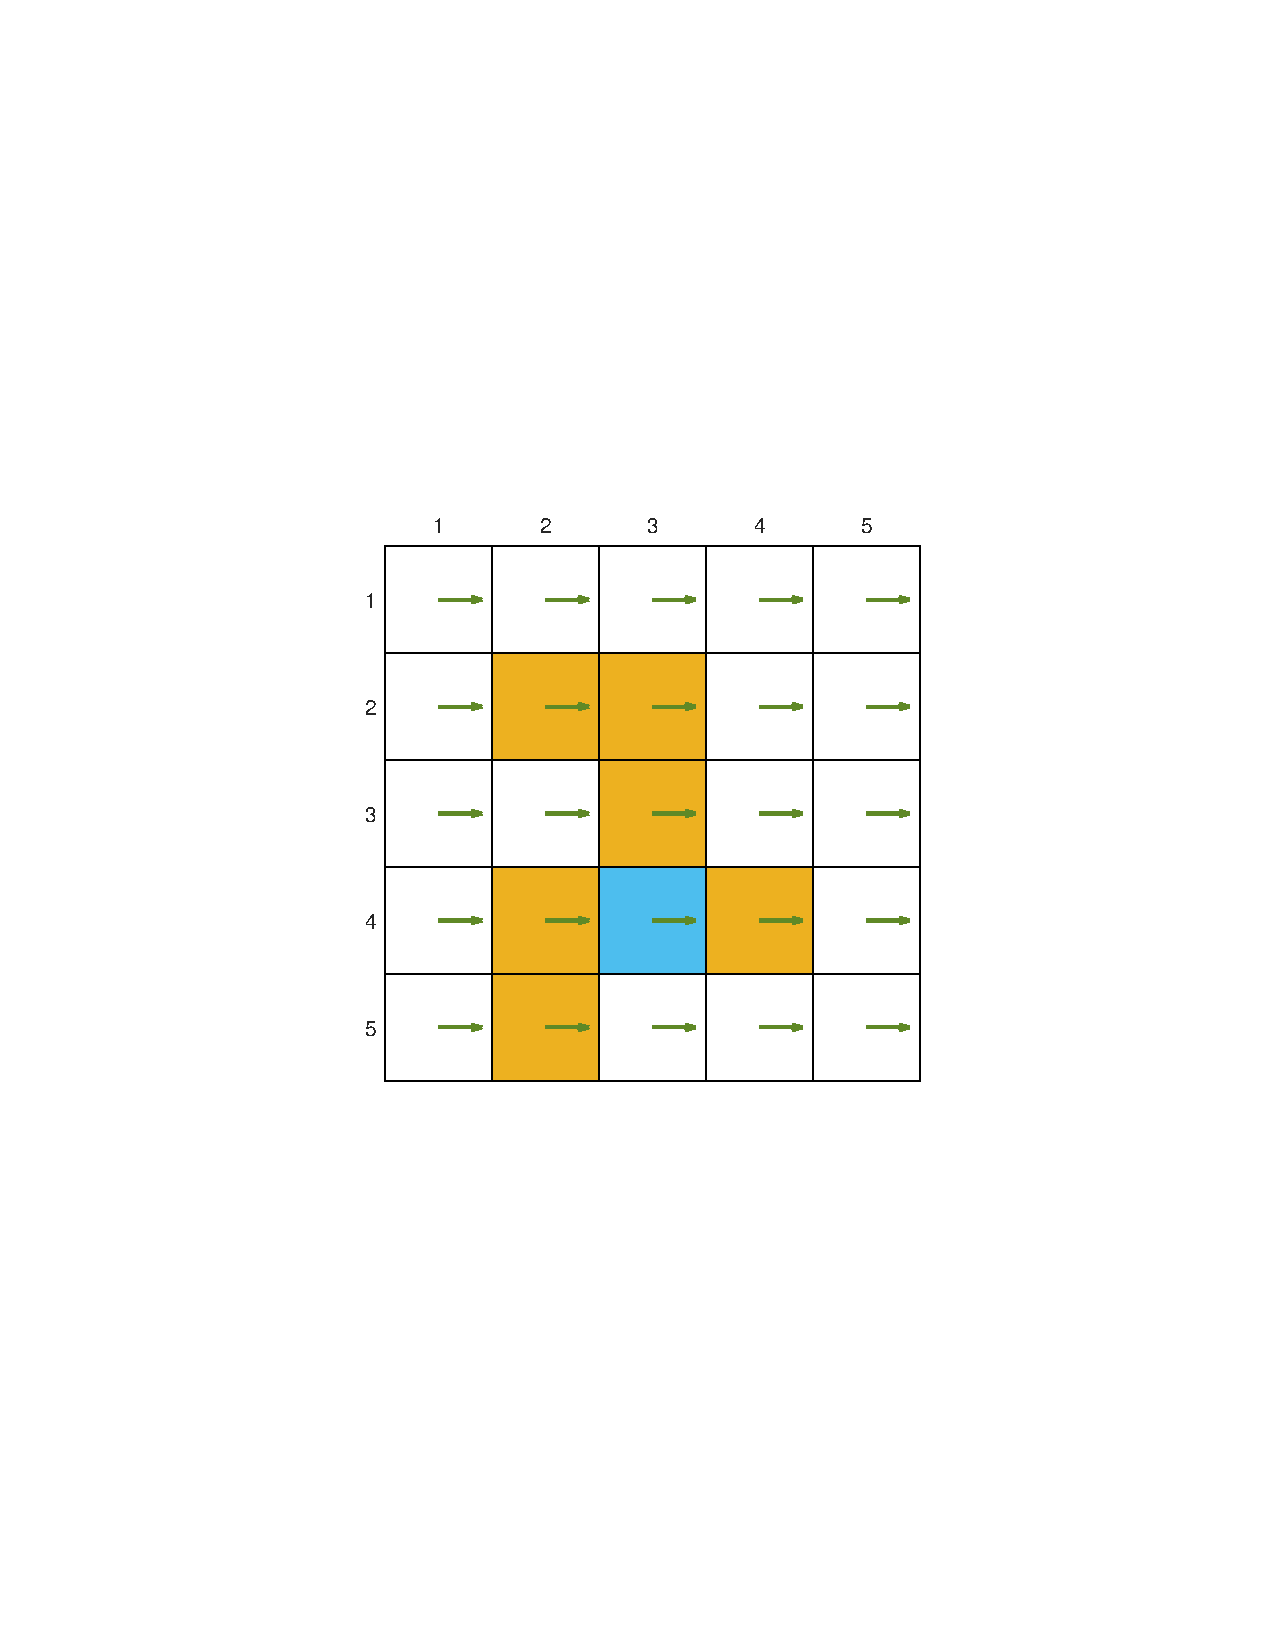
\includegraphics[width=0.25\linewidth]{fig_gridPolicy_moveRight.pdf}
  \includegraphics[width=0.25\linewidth]{fig_gridStateValue_moveRight.pdf}\\
  \vspace{10pt}
  \includegraphics[width=0.25\linewidth]{fig_gridPolicy_random.pdf}
  \includegraphics[width=0.25\linewidth]{fig_gridStateValue_random.pdf}
  \label{figChapterBellman_demoBEandStateValue}
\end{figure}

\end{frame}

\AtBeginSection[]% put it to the start of each section
{
  \begin{frame}
    \frametitle{Outline}
    \tableofcontents[currentsection]
  \end{frame}
}
\section{Action value}
%******************************************************************************
\begin{frame}
\frametitle{Action value}
From state value to action value:
\begin{itemize}
\item State value: the average return the agent can get \emph{starting from a state}.
\pause
\item Action value: the average return the agent can get \emph{starting from a state} and \emph{taking an action}.
\end{itemize}
\pause
Why do we care action value? Because we want to know which action is better. This point will be clearer in the following lectures. We will frequently use action values.

\end{frame}
%******************************************************************************
\begin{frame}
\frametitle{Action value}
Definition:
$$q_{\pi}(s,a)=\E[G_t|S_t=s,A_t=a]$$

\begin{itemize}
\item $q_{\pi}(s,a)$ is a function of the state-action pair $(s,a)$
\item $q_{\pi}(s,a)$ depends on $\pi$
\end{itemize}

\pause
It follows from the properties of conditional expectation that
$$\underbrace{\E[G_t|S_t=s]}_{v_\pi(s)}=\sum_a \underbrace{\E[G_t|S_t=s,A_t=a]}_{q_\pi(s,a)}\pi(a|s)$$
Hence,
\begin{align}\label{eq_statevalueandactionvalue}
\blue{v_{\pi}(s)}=\sum_a \pi(a|s)\blue{q_{\pi}(s,a)}
\end{align}

\end{frame}
%******************************************************************************
\begin{frame}
\frametitle{Action value}
Recall that the state value is given by
\begin{align}\label{eq_MDP_bellmanequationForActionValue}
v_\pi(s)=\sum_{a}\pi(a|s)\Big[\underbrace{\sum_{r}p(r|s,a)r+\gamma  \sum_{s'} p(s'|s,a)v_\pi(s')}_{\blue{q_\pi(s,a)}}\Big]
\end{align}
\pause
By comparing \eqref{eq_statevalueandactionvalue} and \eqref{eq_MDP_bellmanequationForActionValue}, we have the \textbf{action-value function} as
\begin{align}\label{eq_expressionofActionValue}
\blue{q_\pi(s,a)}
&=\sum_{r}p(r|s,a)r+\gamma  \sum_{s'} p(s'|s,a)\blue{v_\pi(s')}
\end{align}

\pause
\eqref{eq_statevalueandactionvalue} and \eqref{eq_expressionofActionValue} are the \blue{two sides of the same coin}:
\begin{itemize}
\item \eqref{eq_statevalueandactionvalue} shows how to obtain state values from action values.
\item \eqref{eq_expressionofActionValue} shows how to obtain action values from state values.
\end{itemize}

\end{frame}
%******************************************************************************
\begin{frame}
\frametitle{Illustrative example for action value}
\begin{figure}[h]
  \centering
  \includegraphics[width=0.3\linewidth]{fig_Bellman_demoReturnPolicy2}
\end{figure}

Write out the action values for state $s_1$:
$$q_\pi(s_1,a_2)=-1+\gamma v_{\pi}(s_2),$$
\pause
Questions:
\begin{itemize}
\item $q_\pi(s_1,a_1),q_\pi(s_1,a_3),q_\pi(s_1,a_4),q_\pi(s_1,a_5)=?$ Be careful!
\end{itemize}
\end{frame}
%******************************************************************************
\begin{frame}
\frametitle{Illustrative example for action value}
\begin{figure}[h]
  \centering
  \includegraphics[width=0.3\linewidth]{fig_Bellman_demoReturnPolicy2}
\end{figure}
For the other actions:
\begin{align*}
q_\pi(s_1,a_1)&=-1+\gamma v_\pi(s_1),\\
q_\pi(s_1,a_3)&=0+\gamma v_\pi(s_3),\\
q_\pi(s_1,a_4)&=-1+\gamma v_\pi(s_1),\\
q_\pi(s_1,a_5)&=0+\gamma v_\pi(s_1).
\end{align*}
\end{frame}
%******************************************************************************
\begin{frame}
\frametitle{Illustrative example for action value}
\begin{figure}[h]
  \centering
  \includegraphics[width=0.3\linewidth]{fig_Bellman_demoReturnPolicy2}
\end{figure}
Highlights:
\begin{itemize}
\item Action value is important since we care about which action to take.
\item We can first calculate all the state values and then calculate the action values.
\item We can also directly calculate the action values with or without models.
\end{itemize}
\end{frame}
\AtBeginSection[]% put it to the start of each section
{
  \begin{frame}
    \frametitle{Outline}
    \tableofcontents[currentsection]
  \end{frame}
}
\section{Summary}
%******************************************************************************
\begin{frame}
\frametitle{Summary}
Key concepts and results:
\begin{itemize}
\item State value: $v_\pi(s)=\E[G_t|S_t=s]$
\item Action value: $q_{\pi}(s,a)=\E[G_t|S_t=s,A_t=a]$
\pause
\item The Bellman equation (elementwise form):
\begin{align*}%\label{eq_MDP_bellmanequation}
{v_\pi(s)}
&=\sum_{a}\pi(a|s)\Big[\underbrace{\sum_{r}p(r|s,a)r+\gamma  \sum_{s'} p(s'|s,a)v_\pi(s')}_{q_\pi(s,a)}\Big]\\
&=\sum_{a}\pi(a|s) q_\pi(s,a)
\end{align*}
\vspace{-10pt}
\pause
\item The Bellman equation (matrix-vector form):
\begin{align*}
{v_\pi=r_\pi+\gamma  P_\pi v_\pi}
\end{align*}
\vspace{-10pt}
\pause
\item How to solve the Bellman equation: closed-form solution, iterative solution
\end{itemize}
\end{frame}


%%%%%%%%%%%%%%%%%%%%%%%%%%%%%%%%%%%%%%%%%%%%%%%%%%%%%%%%%%%%%%%%%%%%%%%%%%%%%%%%%%%%%%%%%%%%%%%%%%
%\bibliographystyle{plainnat}
%\bibliography{myOwnPub,zsyReferenceAll}
\end{document}
